\documentclass[aps,prxquantum,preprint,superscriptaddress,amsmath,amssymb]{revtex4-2}
\usepackage{graphicx}
\graphicspath{{./figures/}}
\usepackage{booktabs}
\usepackage{siunitx}
\usepackage{braket}
\usepackage{xr}
\usepackage[colorlinks=true, citecolor=blue, linkcolor=blue, urlcolor=blue]{hyperref}
\usepackage[capitalize]{cleveref}
\externaldocument[MAIN-]{01_track_B_metrology_main}

\renewcommand{\theequation}{S\arabic{equation}}
\renewcommand{\thefigure}{S\arabic{figure}}
\renewcommand{\thetable}{S\arabic{table}}
\renewcommand{\thesection}{S\arabic{section}}

\setlength{\emergencystretch}{1.5em}
\begin{document}

\title{Supplemental Material:\\The Cavity-Loss Barrier to Ultrastrong-Coupling Quantum Metrology}

\author{Juste Deuyekbe}
\affiliation{Department of Physics, Faculty of Science, University of Ngaoundere, P.O. Box 454, Ngaoundere, Cameroon}

\author{P. Djorw\'e}
\email{djorwepp@gmail.com}
\affiliation{Department of Physics, Faculty of Science, University of Ngaoundere, P.O. Box 454, Ngaoundere, Cameroon}
\affiliation{Stellenbosch Institute for Advanced Study (STIAS), Stellenbosch 7600, South Africa}

\author{A.-H. Abdel-Aty}
\affiliation{Department of Physics, College of Sciences, University of Bisha, Bisha 61922, Saudi Arabia}

\author{A. Elrashidi}
\email{a.elrashidi@ubt.edu.sa}
\affiliation{College of Engineering, University of Business and Technology, Jeddah 21448, Saudi Arabia}

\author{Nsangou Mama}
\email{mnsangou@yahoo.com}
\affiliation{Department of Physics, Faculty of Science, University of Maroua, P.O.Box 46, Maroua, Cameroon}

\author{S. G. Nana Engo}
\email{serge.nana-engo@facsciences-uy1.cm}
\affiliation{Department of Physics, Faculty of Science, University of Yaounde I, P.O.Box 812, Yaounde, Cameroon}

\maketitle

\noindent
This Supplemental Material provides the model definitions and QFI conventions (\cref{sec:si_exact_diag}), numerical convergence (\cref{sec:si_convergence}), the single-qubit and collective loss calculations that produce the main retention values (\cref{sec:si_loss_adjusted,sec:si_dicke_loss}), the cavity-channel HEOM cross-check (\cref{sec:si_cavity_heom}), the multilevel-emitter leakage screen (\cref{sec:si_multilevel}), the finite-size scaling (\cref{sec:si_finite_size}), and the additional model-specific screens and feasibility considerations that support the main-text boundaries (\cref{sec:si_additional,sec:si_feasibility_B}).

% ==================================================================
\section{Model definitions and QFI conventions}
\label{sec:si_exact_diag}

We set $\hbar=1$ throughout. The single-qubit quantum Rabi Hamiltonian is
\begin{equation}
\hat{H}_{\text{Rabi}} = \frac{\omega_q}{2}\hat{\sigma}_z + \omega_c \hat{a}^\dagger \hat{a} + g \hat{\sigma}_x (\hat{a} + \hat{a}^\dagger),
\label{eq:si_rabi}
\end{equation}
with normalized coupling $\eta = g/\omega_c$. The collective Dicke Hamiltonian for $N$ qubits is
\begin{equation}
\hat{H}_{\text{Dicke}} = \omega_c \hat{a}^\dagger \hat{a} + \omega_q \hat{J}_z + \frac{g}{\sqrt{N}} \hat{J}_x (\hat{a} + \hat{a}^\dagger),
\label{eq:si_dicke}
\end{equation}
with $\hat{J}_{x,z} = \frac{1}{2}\sum_{i=1}^N \hat{\sigma}_{x,z}^{(i)}$. The $1/\sqrt{N}$ normalization gives the thermodynamic critical coupling $\eta_c = \frac{1}{2}\sqrt{\omega_q/\omega_c}$, which equals $\num{0.5}$ at resonance.

Both Hamiltonians are diagonalized in the Fock-qubit (or collective-spin) basis with truncations $n_{\max}=\num{50}$ (Rabi) and $n_{\max}=\num{35}$ (Dicke, $N\le\num{64}$). The driven DCE protocol modulates the coupling as $g(t)=g_0+g_d\cos(\omega_d t)$; the Schr\"odinger equation is integrated with QuTiP~\cite{Johansson2012}. Because the interaction is time dependent, strongly nonadiabatic USC control is gauge relative~\cite{Stokes2021}, and the results below are interpreted as effective-control-model predictions, not gauge-independent device forecasts. A controlled finite-dimensional similarity transformation of Hamiltonian, state, control, and observables (see \cref{sec:si_additional}) verifies internal representation consistency to $\num{5e-9}$ but does not resolve the physical gauge ambiguity.

\subsection{Quantum Fisher information}
\label{sec:si_qfi}

For a static eigenstate family $\hat H(\eta)\ket{\Psi_G(\eta)}=E_0(\eta)\ket{\Psi_G(\eta)}$ with generator $\hat H_{\rm int}=\partial_\eta\hat H$, the exact QFI is the gap-weighted sum
\begin{equation}
F_Q = 4\sum_{k\neq 0}\frac{|\braket{\Psi_k|\hat H_{\text{int}}|\Psi_G}|^2}{(E_k-E_0)^2}.
\label{eq:si_qfi_static}
\end{equation}
The variance form $F_Q=4\,\mathrm{Var}[\hat H_{\rm int}]$ holds only for unitary-encoding families and overestimates the static QFI by a factor $\num{3.4}$ at the sampled maximum ($\num{20.9}$ vs.\ $\num{6.116}$ at $\eta=\num{1.14}$). The reported static values are the fidelity-based finite-difference form of \cref{eq:si_qfi_static}, with $\epsilon=\num{1e-4}$; agreement with the exact eigenspectrum form is below \qty{0.21}{\percent} across the USC sweep.

For the driven DCE protocol the state is not stationary, and the QFI is computed from the fidelity
\begin{equation}
F_Q(t) \approx 8\,\frac{1-|\braket{\Psi_\eta(t)|\Psi_{\eta+\delta}(t)}|}{\delta^2},
\qquad \delta=\num{1e-3},
\label{eq:si_qfi_time}
\end{equation}
which becomes exact as $\delta\to0$. All DCE QFI values quoted in the main text are this fidelity-based quantity. At the single-qubit DCE optimum the instantaneous variance form ($\num{4}\,\mathrm{Var}[\hat H_{\rm int}]$) gives \num{225.5}, against the fidelity-based peak of \num{170903}; the two are different quantities and are not interchanged. Convergence with respect to time step and $\delta$ is reported in \cref{sec:si_convergence}.

All values are normalized to the coherent-state baseline $F_Q^{\rm coh}=1$. This baseline does not match the pump power, intracavity population, bandwidth, or readout cost of any driven comparison.

\subsection{Energy budget}
\label{sec:si_energy_budget}

The exact static QFI obeys the reduced budget $F_Q\le 4(2n_{\rm virt}+1)$ with $n_{\rm virt}=\braket{\hat a^\dagger\hat a}_{\Psi_G}$. This bound holds at all 16 points of the regenerated USC sweep, with residuals $4(2n_{\rm virt}+1)-F_Q$ ranging from $\num{+2.50}$ ($\eta=\num{0.7}$) to $\num{+10.39}$ ($\eta=\num{1.3}$). The measured small-$\eta$ asymptote $F_Q\approx 1+3\eta^2$ is consistent with $n_{\rm virt}\approx\eta^2/4$, so the metrological content is carried by the virtual population. Because the single qubit is a two-level system, this budget saturates; the measured curve peaks at $F_Q=\num{6.116}$ at $\eta=\num{1.14}$ and decreases beyond.

% ==================================================================
\section{Numerical convergence}
\label{sec:si_convergence}

\subsection{Fock truncation}

The Rabi QFI is converged to below $\num{1e-6}$ for $n_{\max}\ge\num{30}$ at $\eta=\num{1.14}$. The Dicke QFI for $N=\num{32}$ is converged to below \qty{0.01}{\percent} for $n_{\max}\ge\num{25}$. The collective spin basis reduces the Hilbert space from $2^N$ to $N+1$ and permits exact diagonalization at $N\le\num{64}$.

\subsection{Time-step and finite-difference convergence of the DCE QFI}

At the quoted single-qubit DCE operating point, the fidelity-based peak QFI varies by less than \qty{0.15}{\percent} across time-step refinements $n_{\rm steps}=\num{100}$--$\num{2000}$ (quoted value at $n_{\rm steps}=\num{500}$). At fixed $n_{\rm steps}=\num{500}$, the peak varies by less than \qty{0.40}{\percent} for $\delta$ between $\num{1e-4}$ and $\num{5e-4}$, and by less than \qty{0.12}{\percent} between $\delta=\num{1e-3}$ (quoted value) and $\delta=\num{1e-4}$. The quoted peak is therefore converged in both parameters.

% ==================================================================
\section{Single-qubit DCE under cavity loss}
\label{sec:si_loss_adjusted}

\subsection{Loss sweep and retention}

The single-qubit DCE protocol ($\eta=\num{0.150}$, $g_d/g_0=\num{0.11923}$, $\omega_q/\omega_c=\num{1.027}$, $\omega_d/\omega_c=\num{2.077}$) is propagated under the Lindblad master equation with collapse operator $\sqrt{\kappa}\,a$, Fock truncation $N_{\rm cav}=\num{20}$, initial state $\ket{0}\otimes\ket{\downarrow}$, and fidelity-based QFI with $\delta=\num{1e-3}$. \Cref{tab:si_loss_adjusted} reports the peak and late-window QFI versus $\kappa$.

\begin{table}[hbt!]
\centering
\caption{Loss-adjusted single-qubit DCE QFI. Reference pure-state peak: \num{170903}.}
\label{tab:si_loss_adjusted}
\begin{tabular}{c c c c c}
\toprule
{$\kappa/\omega_c$} & {$\kappa/2\pi$ (MHz)} & {Peak QFI} & {Late-window avg} & {Percent of pure (peak)} \\
\midrule
\num{0}       & \num{0}     & \num{170903} & \num{132800} & \qty{100}{\percent} \\
\num{1e-5}   & \num{0.06}  & \num{133806} & \num{100003} & \qty{78}{\percent} \\
\num{5e-5}   & \num{0.3}   & \num{134693} & \num{100977} & \qty{79}{\percent} \\
\num{1e-4}   & \num{0.6}   & \num{137772} & \num{104482} & \qty{81}{\percent} \\
\num{5e-4}   & \num{3}     & \num{119926} & \num{96606}  & \qty{70}{\percent} \\
\num{1e-3}   & \num{6}     & \num{82687}  & \num{71075}  & \qty{48}{\percent} \\
\num{5e-3}   & \num{30}    & \num{11653}  & \num{6287}   & \qty{6.8}{\percent} \\
\num{1e-2}   & \num{60}    & \num{5957}   & \num{1919}   & \qty{3.5}{\percent} \\
\num{2e-2}   & \num{120}   & \num{3376}   & \num{853}    & \qty{2.0}{\percent} \\
\num{4.1e-2} & \num{246}   & \num{1640}   & \num{406}    & \qty{0.96}{\percent} \\
\bottomrule
\end{tabular}
\end{table}

The retention is not monotonic over the three lowest-loss rows (\qty{78}{\percent}, \qty{79}{\percent}, \qty{81}{\percent}). The first sampled row at or above \qty{80}{\percent} retention is $\kappa/\omega_c=\num{1e-4}$ ($\kappa/2\pi=\qty{0.6}{\mega\hertz}$); no continuous threshold is inferred. At the simulated physical operating point $\kappa/\omega_c=\num{4.1e-2}$ ($\kappa/2\pi\approx\qty{246}{\mega\hertz}$; the cited CPW reference is approximately \qty{248}{\mega\hertz}), retention is $\sim\qty{1}{\percent}$ of the pure-state peak. The degradation exceeds the simple envelope $\exp(-\kappa t)$ because the Lindblad dynamics modify the full state evolution, not just the peak amplitude.

\subsection{Continuous $\kappa$ sweep}
\label{sec:si_kappa_sweep}

A ten-point log-spaced sweep of $\kappa/\omega_c\in\{0,\num{1e-5},\num{3e-5},\num{1e-4},\num{3e-4},\num{1e-3},\num{3e-3},\num{1e-2},\num{2e-2},\num{4.1e-2}\}$ (\num{500} output samples per point) plateaus at $0.78$--$0.81$ retention for $\kappa/\omega_c\le\num{3e-4}$, then falls to $0.484$ at $\num{1e-3}$, $0.117$ at $\num{3e-3}$, $0.035$ at $\num{1e-2}$, and $0.010$ at the physical $\kappa$. Log-linear interpolation gives the crossovers $\kappa^{\ast}_{80}=\num{1.45e-4}$ and $\kappa^{\ast}_{50}=\num{9.38e-4}$. The \qty{80}{\percent} crossover sits at the plateau edge and is mildly sensitive to the $\num{1e-4}$ bump; the \qty{50}{\percent} crossover is robust to it.

\subsection{Combined cavity, qubit-$T_1$, and temperature row}
\label{sec:si_joint_row}

A single master-equation row combines, at the same operating point, the finite-temperature drive ($T=\qty{20}{\milli\kelvin}$), physical cavity loss ($\kappa/\omega_c=\num{4.1e-2}$), and a conservative qubit-relaxation benchmark ($\gamma_1/\omega_c=\num{1e-4}$), with $N_{\rm cav}=\num{10}$ over $20$ drive periods. The pure-state peak is $\num{30418}$ and the joint peak is $\num{1637}$, an end-to-end retention of \qty{5.4}{\percent}. The joint loss-dominated peak matches the $\kappa$-sweep value at the same $\kappa$ ($\num{1640}$) to within \qty{0.2}{\percent}, confirming cavity decay as the dominant channel. The row is joint in (temperature $\times$ loss $\times$ $T_1$) at the two-level emitter truncation; a multilevel merge remains an open follow-up.

\subsection{Combined cavity and qubit dissipation}
\label{sec:si_qubit_loss}

The conservative transmon-like benchmark at $\omega_c/2\pi=\qty{6}{\giga\hertz}$ ($T_1=\qty{30}{\micro\second}$, $T_\phi=\qty{5}{\micro\second}$) gives dimensionless rates $\gamma_1/\omega_c=\num{8.84e-7}$ and $\gamma_\phi/\omega_c=\num{5.31e-6}$. Without cavity loss the qubit channels retain \qty{78.56}{\percent} ($T_1$ alone), \qty{79.08}{\percent} ($T_\phi$ alone), and \qty{79.08}{\percent} ($T_1$ and $T_\phi$ together). At the physical cavity-loss point plus both qubit channels, retention is \qty{0.9594}{\percent}, essentially identical to cavity loss alone. Cavity decay is the dominant channel over the tested window.

% ==================================================================
\section{Collective Dicke+DCE under cavity loss}
\label{sec:si_dicke_loss}

\subsection{Reduced-truncation loss matrix}

The Dicke+DCE operating point ($N=\num{32}$, $\eta=\num{1.15}$, $g_d/g_0=\num{0.15}$, $\omega_q/\omega_c=\num{1.0}$, $\omega_d/\omega_c=\num{2.0}$) is propagated under Lindblad single-photon cavity loss at photon truncations $N_{\rm cav}=\num{6},\num{8},\num{10},\num{12}$ and $\kappa/\omega_c\in\{0,\num{1e-4},\num{1e-3},\num{1e-2},\num{4.1e-2}\}$, with $\texttt{atol}=\texttt{rtol}=\num{1e-10}$ and $n_{\rm steps}=\num{200}$ over ten drive periods. Every stored state satisfies the trace, Hermiticity, and eigenvalue criteria (worst minimum eigenvalue $-\num{1.34e-5}$ against the $-\num{1e-4}$ floor).

\begin{table}[hbt!]
\centering
\caption{Loss-adjusted Dicke+DCE QFI at $N_{\rm cav}=\num{6}$ (Hilbert dim 198). Reference pure-state peak: \num{2962}.}
\label{tab:si_dicke_loss}
\begin{tabular}{c c c c c}
\toprule
{$\kappa/\omega_c$} & {$\kappa/2\pi$ (MHz)} & {Peak QFI} & {Late-window avg} & {Retained} \\
\midrule
\num{0}       & \num{0}     & \num{2962}  & \num{2594} & :  \\
\num{1e-4}   & \num{0.6}   & \num{2927}  & \num{2566} & \qty{99}{\percent} \\
\num{1e-3}   & \num{6}     & \num{2828}  & \num{2490} & \qty{95}{\percent} \\
\num{1e-2}   & \num{60}    & \num{1818}  & \num{1678} & \qty{61}{\percent} \\
\num{4.1e-2} & \num{246}   & \num{474}   & \num{321}  & \qty{16}{\percent} \\
\bottomrule
\end{tabular}
\end{table}

\subsection{Truncation dependence}

Retention is truncation-dependent and not converged. The full trend at the physical $\kappa$ is shown in \cref{tab:si_dicke_loss_convergence}.

\begin{table}[hbt!]
\centering
\caption{Truncation dependence of Dicke+DCE QFI retention at the physical cavity linewidth. Retention is relative to each truncation's own zero-loss peak.}
\label{tab:si_dicke_loss_convergence}
\begin{tabular}{c c c c c}
\toprule
{$N_{\rm cav}$} & {Hilbert dim} & {Peak QFI ($\kappa=0$)} & {Peak QFI (physical $\kappa$)} & {Retention} \\
\midrule
\num{6}  & \num{198} & \num{2962}  & \num{474}  & \qty{16}{\percent} \\
\num{10} & \num{330} & \num{2363}  & \num{290}  & \qty{12}{\percent} \\
\num{12} & \num{396} & \num{4833}  & \num{320}  & \qty{7}{\percent}  \\
\num{16} & \num{528} & \num{5786}  & \num{255}  & \qty{4.4}{\percent} \\
\num{20} & \num{660} & \num{9851}  & \num{265}  & \qty{2.7}{\percent} \\
\num{24} & \num{792} & \num{10584} & \num{273}  & \qty{2.6}{\percent} \\
\bottomrule
\end{tabular}
\end{table}

The non-monotonic pure-state peak ($\num{2962}\to\num{2363}\to\num{4833}\to\num{5786}\to\num{9851}\to\num{10584}$) reflects Fock-space confinement at the smallest truncation. Retention decreases monotonically. Of the six truncation comparisons against the larger truncation ($N_{\rm cav}=\num{16}\to\num{24}$ and $\num{20}\to\num{24}$ at each of the three loss values), two meet the \qty{5}{\percent} tolerance ($\num{16}\to\num{24}$ at $\kappa/\omega_c=\num{1e-2}$, $\num{20}\to\num{24}$ at the physical $\kappa$); the rest exceed it. The physical-point retention is therefore a truncation-dependent range of roughly \qty{16}{\percent} ($N_{\rm cav}=\num{6}$) down to \qty{2.6}{\percent} ($N_{\rm cav}=\num{24}$), not a converged number.

\subsection{Boundary-peak convergence}
\label{sec:si_dicke_convergence}

Extending the pure-state Dicke+DCE time trace at $N_{\rm cav}=\num{6}$ to periods $\num{20}$--$\num{60}$ shows the peak QFI continues to grow monotonically and occurs at the last stored time point for every window (\cref{tab:si_dicke_convergence}). The quoted boundary value $\num{251557}\times$ at $N_{\rm cav}=\num{28}$ and $T_{\max}=\num{40}$ is therefore an arbitrary cutoff, not a converged local maximum.

\begin{table}[hbt!]
\centering
\caption{Dicke+DCE boundary-peak convergence at $N_{\rm cav}=\num{6}$. The peak occurs at the last stored time point for every window.}
\label{tab:si_dicke_convergence}
\begin{tabular}{c c c}
\toprule
{$T_{\rm max}$ (periods)} & {Peak QFI} & {Late-window avg} \\
\midrule
\num{20} & \num{9932}  & \num{8219}  \\
\num{30} & \num{19093} & \num{16060} \\
\num{40} & \num{33109} & \num{27535} \\
\num{50} & \num{48328} & \num{39760} \\
\num{60} & \num{69475} & \num{57117} \\
\bottomrule
\end{tabular}
\end{table}

\subsection{Photon-sector decomposition}

Replaying the validated Dicke+DCE rows and projecting onto the $n\le n_{\rm cut}$ sector shows the low-photon blocks carry the parameter-relevant coherence. At $N_{\rm cav}=\num{6}$ ($\langle n\rangle=\num{2.9}$--$\num{3.5}$) the $n\le\num{2}$ sector peak exceeds the full-space peak ($\num{2.65}\times$ at $\kappa=0$, $\num{1.28}\times$ at the physical $\kappa$) while retaining only \qty{33}{\percent}--\qty{37}{\percent} trace weight; the overshoot decreases monotonically to $1.000$ as $n_{\rm cut}\to N_{\rm cav}$. At $N_{\rm cav}=\num{12}$ the sector curve converges monotonically with the cutoff (\cref{tab:si_photon_sector}), and at the physical $\kappa$ the $n_{\rm cut}=\num{10}$ projection (\qty{84}{\percent} weight) is within \qty{0.1}{\percent} of the full peak.

\begin{table}[hbt!]
\centering
\caption{Fraction of the full-space peak QFI retained by the $n\le n_{\rm cut}$ photon sector at $N_{\rm cav}=\num{12}$; trace weight in parentheses.}
\label{tab:si_photon_sector}
\begin{tabular}{lrrrrr}
\toprule
$n_{\rm cut}$ & \num{4} & \num{6} & \num{8} & \num{10} & \num{12} \\
\midrule
$\kappa/\omega_c=\num{1e-2}$ & $0.791\,(0.34)$ & $0.860\,(0.51)$ & $0.897\,(0.67)$ & $0.946\,(0.83)$ & $1.000\,(1.00)$ \\
$\kappa/\omega_c=\num{4.1e-2}$ & $0.753\,(0.38)$ & $0.925\,(0.54)$ & $0.988\,(0.69)$ & $1.001\,(0.84)$ & $1.000\,(1.00)$ \\
\bottomrule
\end{tabular}
\end{table}

Sector QFI is not additive across sectors, so the $N_{\rm cav}=\num{6}$ overshoot is a projection effect. The curves are a truncation-sensitivity diagnostic, not a decomposition of the full QFI into independent contributions.

% ==================================================================
\section{Cavity-channel HEOM cross-check}
\label{sec:si_cavity_heom}

The Markovian cavity-loss treatment underlying the retention values in \cref{sec:si_loss_adjusted,sec:si_dicke_loss} is cross-checked against a cavity-mode HEOM calculation: a Fock-space mode ($d=\num{12}$) coupled through the position quadrature $\hat x=\hat a+\hat a^\dagger$ to a structured Drude--Lorentz bath and benchmarked against $\sqrt{\kappa}\hat a$ Lindblad. The grid spans $\kappa/\omega_c\in\{\num{1e-4},\num{4.1e-2}\}$, Drude cutoffs $\gamma/\omega_c\in\{\num{5},\num{10},\num{20},\num{40}\}$, hierarchy depths $L=\num{2},\num{3},\num{4}$, temperatures $T=\num{0.01},\num{0.05}$, and windows $t_{\rm final}=\num{1},\num{2}$ (\num{96} rows).

At $\kappa/\omega_c=\num{1e-4}$ all \num{18} physical rows give mean fidelity errors of $\num{9.2e-5}$--$\num{3.7e-4}$; the hierarchy shows no depth dependence, confirming that Markovian and non-Markovian dynamics are indistinguishable at this linewidth. At $\kappa/\omega_c=\num{4.1e-2}$ the \num{18} physical rows give mean fidelity errors of \qty{4.8}{\percent}--\qty{24}{\percent} depending on the Drude cutoff and time window; the hierarchy converges at depth $L=\num{3}$. The \num{60} remaining rows fail the positivity criterion (minimum eigenvalue down to $-\num{1.4}$), documenting a genuine numerical limitation of the HEOM hierarchy for strong cavity-bath coupling.

The Markovian treatment is therefore approximate at the physical linewidth: the retention values should be read as first-order Markovian estimates whose sensitivity to cavity-bath memory is a tested model-comparison range of approximately \qty{4.8}{\percent}--\qty{24}{\percent}, not a propagated statistical uncertainty.

% ==================================================================
\section{Multilevel-emitter leakage}
\label{sec:si_multilevel}

The two-level approximation used in the main-text QFI computations is tested against a common oscillator-based emitter interface parameterized by declared transition-frequency ratios for three effective spectra: transmon-like, flux-qubit-like, and fluxonium-like. Each retains $d_e=\num{2},\dots,\num{5}$ emitter levels. Static rows use $\eta=\num{0.15}$ and $\num{1.0}$; driven rows use drive coefficients $g_d=\num{0.11923}$ (reference) and $\num{0.5}$ (strong) at $\kappa/\omega_c=0$ and $\num{4.1e-2}$ over \num{40} drive periods. The adequacy criterion is declared before scanning: maximum leakage to levels $\ket{2}$ and above below \qty{1}{\percent} over the window.

No driven $d_e\ge\num{3}$ row meets the criterion at the reference drive. Window-maximum leakage ranges from \qty{2.99}{\percent} (fluxonium-like, $d_e=\num{3}$) to \qty{81.5}{\percent} (fluxonium-like, $d_e=\num{5}$, strong drive). Paired two-level versus multilevel comparisons show the multilevel peak QFI relative change from the two-level baseline ranging from $-0.873$ to $+7.36$, with the largest positive deviations at strong drive where leakage is largest.

A staged drive-amplitude sweep over $g_d\in\{0,\num{0.02},\num{0.04},\num{0.06},\num{0.08},\num{0.10},\num{0.11923}\}$ at $d_e=\num{3}$ (\num{42} rows, $\kappa/\omega_c=0$ and $\num{4.1e-2}$) identifies platform-specific safe operating windows at physical loss (\cref{tab:si_multilevel_sweep}). The QFI enhancement at those leakage-acceptable points is orders of magnitude below the reference value.

\begin{table}[hbt!]
\centering
\caption{Maximum drive coefficient $g_d$ satisfying the \qty{1}{\percent} leakage criterion at physical loss ($d_e=\num{3}$, \num{40} drive periods) and the corresponding peak QFI for the coupling estimand.}
\label{tab:si_multilevel_sweep}
\begin{tabular}{l c c}
\toprule
{Platform} & {Max $g_d$} & {Peak QFI} \\
\midrule
Fluxonium-like & $\num{0.06}$ & $\num{85.5}$ \\
Flux-qubit-like & $\num{0.04}$ & $\num{77.5}$ \\
Transmon-like & $\num{0.02}$ & $\num{54.2}$ \\
\bottomrule
\end{tabular}
\end{table}

The trade-off between leakage and QFI enhancement is monotonic. The \qty{1}{\percent} criterion is a model choice, and the models are declared effective spectra, not device simulations.

% ==================================================================
\section{Finite-size scaling of the Dicke model}
\label{sec:si_finite_size}

The exact static Dicke ground-state QFI is evaluated at two cavity truncations per size bracket for $N=\num{4},\dots,\num{64}$ at $\omega_q/\omega_c=\num{1.0}$ and $\num{1.005}$ (\num{52} rows). All static rows are truncation-converged (relative change below \qty{5}{\percent}; typical values $10^{-11}$--$10^{-14}$). The static QFI at $N=\num{32}$, $\omega_q/\omega_c=\num{1.0}$ is \num{228.6}, reproducing the reference value.

Descriptive power-law fits over $N\in[\num{6},\num{18}]$ give $\alpha=\num{2.197}\pm\num{0.039}$ ($\omega_q/\omega_c=\num{1.0}$, $R^2=\num{0.9984}$) and $\alpha=\num{2.216}\pm\num{0.034}$ ($\omega_q/\omega_c=\num{1.005}$, $R^2=\num{0.9988}$), consistent with the historical $\alpha=\num{2.21}$. Dropping the largest in-range point changes $\alpha$ by only \num{0.004}. Beyond $N\approx\num{21}$ the local growth exponent falls below unity (\num{0.67} at $N=\num{24}$, \num{0.34} at $N=\num{27}$) before recovering to \num{0.85} at $N=\num{64}$. Single-plateau saturated forms do not describe the data over $N\in[\num{4},\num{64}]$, so no saturation plateau is reached up to $N=\num{64}$ within this grid. The fits are recorded with uncertainty intervals and boundary sensitivity; they are explicitly descriptive.

Driven Dicke+DCE rows at $N_{\rm cav}=\num{6}$ show the lossless peak growing from \num{785} ($N=\num{4}$) to \num{1852} ($N=\num{12}$) and \num{2768} ($N=\num{24}$) at a fixed pump proxy $g_d^2=\num{0.0298}$. Cavity loss reduces the peak and moves it into the window (\cref{tab:si_finite_size}).

\begin{table}[hbt!]
\centering
\caption{Driven Dicke+DCE resource-accounting at $g_d^2=\num{0.0298}$ ($N_{\rm cav}=\num{6}$). Emitted proxy is $\kappa\int n(t)\,dt$, not a measured output.}
\label{tab:si_finite_size}
\begin{tabular}{c c c c c c}
\toprule
{$N$} & {$\kappa/\omega_c$} & {Peak $F_Q$} & {Peak period} & {Max $\bar n$} & {Emitted proxy} \\
\midrule
\num{4}  & \num{0}      & \num{785.3} & \num{10.0} & \num{3.25} & \num{0}     \\
\num{4}  & \num{1e-2}   & \num{469.3} & \num{10.0} & \num{3.17} & \num{0.663} \\
\num{4}  & \num{4.1e-2} & \num{96.0}  & \num{6.8}  & \num{3.06} & \num{2.394} \\
\num{12} & \num{0}      & \num{1851.6}& \num{10.0} & \num{3.19} & \num{0}     \\
\num{12} & \num{1e-2}   & \num{1072.6}& \num{10.0} & \num{2.90} & \num{0.696} \\
\num{12} & \num{4.1e-2} & \num{188.6} & \num{7.7}  & \num{2.70} & \num{2.830} \\
\num{24} & \num{0}      & \num{2768.1}& \num{10.0} & \num{2.94} & \num{0}     \\
\bottomrule
\end{tabular}
\end{table}

The screen supports a descriptive superlinear finite-size trend over the declared interval, with uncertainty and boundary sensitivity reported; it establishes no thermodynamic exponent, no phase transition, and no restored global bound. The resource accounting is a partial pump/emitted-photon proxy comparison, not a jointly matched operational advantage.

Companion eta-sweep curves at $N=\num{4},\num{8},\num{16},\num{32}$ (produced by the same physics core and anchored at $\eta=\num{1.15}$ against the finite-size grid to below $\num{3e-7}$ relative deviation) show the sampled static-QFI maximum shifting with $N$ ($\approx\num{1.40}$ at $N=\num{4}$, $\approx\num{1.15}$ at $N=\num{16}$, $\approx\num{1.10}$ at $N=\num{32}$). The tabulated $\eta=\num{1.15}$ operating point is therefore not the sampled optimum for every $N$.

% ==================================================================
\section{Additional model-specific screens}
\label{sec:si_additional}

The following screens bound the operational significance of the main-text QFI values but are not the central results. They are grouped here to keep the main text focused.

\subsection{Thermal-competition screen}
\label{sec:si_thermal}

A finite-temperature Lindblad screen over $T\in[\num{10},\num{200}]~\unit{\milli\kelvin}$ and $\omega_c/2\pi\in[\num{5},\num{8}]~\unit{\giga\hertz}$ uses explicit emission and absorption channels $L_-=\sqrt{\kappa(n_{\rm th}+1)}a$, $L_+=\sqrt{\kappa n_{\rm th}}a^\dagger$ with $n_{\rm th}$ evaluated at the declared cavity frequency, plus separate qubit-thermalization rows. The retention criterion is the first sampled temperature at which peak QFI relative to the same-configuration zero-temperature reference falls below \qty{80}{\percent}.

For the reference driven row ($\eta=\num{0.15}$, vacuum initial state, $\kappa/\omega_c=\num{4.1e-2}$, $\omega_c/2\pi=\qty{6}{\giga\hertz}$), the zero-temperature peak QFI is \num{1642.1}, retention is \num{0.985} at \qty{50}{\milli\kelvin} and \num{0.775} at \qty{100}{\milli\kelvin}, so the sampled crossover is at \qty{100}{\milli\kelvin}. The cavity Bose--Einstein occupation is $\num{5.6e-7}$ at \qty{20}{\milli\kelvin} and \num{5.95e-2} at \qty{100}{\milli\kelvin}. The screen is a sampled retention criterion under the declared bath and preparation; it is not a universal temperature threshold.

\subsection{Homodyne output-field CFI screen}

An idealized joint-system QFI does not by itself specify a laboratory readout. A bounded output-field screen uses the input--output convention $a_{\rm out}(t)=a_{\rm in}(t)+\sqrt{\kappa_{\rm ext}}a(t)$ with vacuum input and $\kappa=\kappa_{\rm ext}+\kappa_{\rm int}$; only the external fraction is treated as monitored output. The measured temporal mode is flat over \num{6} or \num{10} drive periods, with a Gaussian quadrature distribution. Among rows with a valid same-state comparison, $F_C/F_Q$ ranges from $0$ to \num{0.603}; the largest static ratio is \num{0.0455}. Historical proposals of \qty{92.4}{\percent} static and \qty{88.1}{\percent} driven are not reproduced. This is a finite-model Gaussian-readout result, not optimized matched-filter CFI or experimental QFI saturation.

\subsection{Multiparameter QFI and representation consistency}
\label{sec:si_multiparameter}

Directional sensitivity is evaluated for the parameter vector $(\eta,\omega_q/\omega_c,g_d/g_0,\phi)$ in the driven protocol and $(\eta,\omega_q/\omega_c)$ for static ground states, using phase-aligned central finite differences at steps $\num{1e-2}$--$\num{1e-4}$. All \num{18} rows are finite, positive semidefinite within tolerance, and converged. At the reference \num{10}-period row and $N_{\rm cav}=\num{20}$, the coupling diagonal is approximately $\num{1.15e3}$ and the nuisance-projected effective coupling information is approximately $\num{4.08e2}$. Driven condition numbers are of order $\num{1e3}$.

A controlled similarity transformation $U=\exp[-i\num{0.37}a^\dagger a]$ at $N_{\rm cav}=\num{30}$ transforms the Hamiltonian, initial state, control, and observables together; unitarity error is \num{1.6e-15}, transformed-state infidelity below \num{4e-16}, and the relative QFI-metric difference is \num{4.8e-9}. This verifies the implemented finite-dimensional similarity transformation; it does not establish agreement between arbitrary laboratory gauges with independently specified controls.

\subsection{Interrogation-window crossover}
\label{sec:si_interrogation}

At the fixed single-qubit DCE operating point, the fidelity-based QFI and the information-rate objective $R_Q(t)=F_Q(t)/t$ are evaluated over \num{40} drive periods for $\kappa/\omega_c\in\{0,\num{1e-4},\num{1e-3},\num{5e-3},\num{1e-2},\num{2e-2},\num{4.1e-2}\}$. At $\kappa/\omega_c\le\num{1e-3}$ both metrics remain boundary-limited; at larger loss the $R_Q$ maximum moves earlier (\num{18.08}, \num{14.00}, \num{10.96}, \num{6.96} periods at $\kappa/\omega_c=\num{0.005},\num{0.01},\num{0.02},\num{0.041}$) with corresponding $F_Q$ falling from \num{10449} to \num{1242} (\cref{tab:si_interrogation}). The stored entropy derivative is a finite-difference mixedness diagnostic, not a thermodynamic entropy-production rate; the crossover is model-specific, not a universal or thermodynamically derived optimum.

\begin{table}[hbt!]
\centering
\caption{Information-rate maxima for the single-qubit DCE protocol.}
\label{tab:si_interrogation}
\begin{tabular}{c c c c c}
\toprule
{$\kappa/\omega_c$} & {$\kappa/2\pi$ (MHz)} & {$t/T_d$ at $R_Q$ max} & {$F_Q$ at max} & {Window status} \\
\midrule
\num{0}      & \num{0}   & \num{40.00} & \num{170670} & boundary \\
\num{1e-4}   & \num{0.6} & \num{40.00} & \num{161087} & boundary \\
\num{1e-3}   & \num{6}   & \num{40.00} & \num{84830}  & boundary \\
\num{5e-3}   & \num{30}  & \num{18.08} & \num{10449}  & interior \\
\num{1e-2}   & \num{60}  & \num{14.00} & \num{5510}   & interior \\
\num{2e-2}   & \num{120} & \num{10.96} & \num{2961}   & interior \\
\num{4.1e-2} & \num{246} & \num{6.96}  & \num{1242}   & interior \\
\bottomrule
\end{tabular}
\end{table}

\subsection{Matched-photon and adaptive-protocol references}
\label{sec:si_matched}

At matched intracavity photon budget $n=\num{9.01}$ (the DCE peak), the pure-state DCE QFI is $\num{4742}\times$ the coherent-state shot-noise reference $F_Q=4n$ and $\num{249}\times$ the squeezed-state reference $F_Q=4n(1+2n)$. Photon-number matching does not match pump power, bandwidth, preparation, loss, readout, or observation time, so these ratios are not device-level advantages. Under cavity loss the DCE QFI collapses as quantified in \cref{sec:si_loss_adjusted}.

A formal comparison with adaptive protocols is retained only as a reference at the DCE peak photon budget and the DCE time-average budget. The adaptive entries are uncertainty-bound or formal-reference expressions, whereas the DCE entries are QFI values, so no cross-estimand enhancement ratios are reported. A physically relevant comparison would require a common estimation task, prior, observation time, loss model, drive budget, and readout; that comparison is outside the present study.

\subsection{Finite-window Floquet-stability screen}

A deterministic screen at the driven single-qubit Rabi model ($\omega_q/\omega_c=\num{1.027}$, $g(t)=g_0[1+(g_d/g_0)\cos(\omega_d t+\phi)]$, cavity loss $\kappa$) evaluates coupling-estimand QFI from paired trajectories at $\eta$ and $\eta+\delta\eta$, with $\delta\eta=\num{1e-3}$. Tier 1 uses $N_{\rm cav}=\num{12},\num{20}$ and \num{40} periods over \num{108} parameter rows; Tier 2 validates five representative rows at \num{80} periods and $N_{\rm cav}=\num{20},\num{30}$. All trajectories satisfy the trace, Hermiticity, and eigenvalue criteria.

Tier 1 classifies \num{79} rows as showing boundary growth and \num{29} as bounded within the screen; no row exceeds the \qty{10}{\percent} truncation-difference criterion. Tier 2 resonant/low-loss rows continue to grow at the boundary, whereas two selected lossy rows remain bounded and agree between the two truncations to better than $10^{-6}$ in peak QFI. The persistence of boundary growth in low-loss resonant rows rejects the claim that two-level saturation is a general passive Floquet stabilizer. The screen is finite-window; no asymptotic stability or phase stability is established.

\subsection{HEOM cross-checks (qubit bath)}
\label{sec:si_heom}

Two HEOM comparisons bound the Lindblad working model for the qubit-bath channel.

\textit{Local short-time check.} A Drude--Lorentz bath ($\omega_q=\num{1.0}$, $\gamma_{\rm cut}=\num{20}$, $\lambda=\num{0.02}$, $\Gamma=\num{0.012535}$, $T=\num{0.001}$, hierarchy depth \num{3}, \num{50} time points to $t_{\rm final}=\num{1.0}$) gives a mean Uhlmann-fidelity error of \qty{1.18}{\percent} (maximum \qty{2.43}{\percent}), all sampled points below \qty{5}{\percent}.

\textit{Extended check.} A hierarchy-depth, temperature, coupling, cutoff, and window sweep (\num{18} rows, \num{15} physical, \num{3} inconclusive) confirms hierarchy convergence at $L=\num{2}$ (relative change \num{4.3e-6} from $L=\num{2}$ to \num{5}). Baseline agreement is \num{5.3e-4} mean, \num{6.6e-4} maximum. Two driven DCE-ratio rows give QFI relative differences of \qty{1.05}{\percent} and \qty{1.09}{\percent} at $\eta_d=\num{0.15}$ and \num{0.10}. The $T=\num{0.35}$ row shows a larger mean error (\qty{7.7}{\percent}), retained as a temperature-scope caveat.

Neither HEOM check validates the driven high-QFI traces; both support the working Lindblad model for their declared scope only.

% ==================================================================
\section{Experimental feasibility}
\label{sec:si_feasibility_B}

\Cref{tab:si_experimental_feasibility} compares the model target with the demonstrated state of the art at the key parameters.

\begin{table}[hbt!]
\centering
\caption{Experimental feasibility assessment.}
\label{tab:si_experimental_feasibility}
\begin{tabular}{l c c c}
\toprule
\textbf{Requirement} & \textbf{Model target} & \textbf{CPW (current USC)} & \textbf{3D cavity (candidate)} \\
\midrule
Number of qubits $N$ & \num{32} & \num{4} \cite{Yoshihara2017} & \num{1} \cite{FornDiaz2017} \\
Coupling $\eta$ & \num{1.15} & \num{1.3} \cite{Niemczyk2010} & \numrange{0.1}{0.3} \cite{FornDiaz2017} \\
Coupling $g/2\pi$ & \qty{6.9}{\giga\hertz} & \qty{6}{\giga\hertz} \cite{Niemczyk2010} & \qty{0.3}{\giga\hertz} \cite{FornDiaz2017} \\
DCE drive $g_d/2\pi$ & \qty{1.0}{\giga\hertz} &, &, \\
Drive frequency $\omega_d/2\pi$ & \qty{12}{\giga\hertz} & Standard & Standard \\
Temperature & $<\qty{200}{\milli\kelvin}$ & \qty{10}{\milli\kelvin} & \qty{10}{\milli\kelvin} \\
Cavity $\kappa/2\pi$ & $<\qty{1}{\mega\hertz}$ & \qty{248}{\mega\hertz} & \qty{0.1}{\mega\hertz} \\
Coherence $T_1$ & $\gg\qty{83}{\nano\second}$ & \qtyrange{10}{100}{\micro\second} & \qtyrange{10}{100}{\micro\second} \\
Floquet bound-state rescue & demonstrable at $\kappa/\omega\sim\num{4e-2}$ & emitter-local only~\cite{Bai2023} & unshown for cavity leakage \\
\bottomrule
\end{tabular}
\end{table}

No demonstrated platform simultaneously satisfies (i) the $\eta=\num{1.15}$ coupling needed for the superradiant collective enhancement, (ii) the sampled single-qubit reference point $\kappa/2\pi=\qty{0.6}{\mega\hertz}$ at which the loss sweep first reaches \qty{80.6}{\percent} retention, and (iii) the uniform collective coupling of $N=\num{32}$ qubits. The cited CPW example provides strong coupling and a partial collective architecture at $\kappa/2\pi\approx\qty{248}{\mega\hertz}$; the cited 3D-cavity example provides the low-linewidth regime at the single-qubit level.

\textit{Platform candidates.} Flux qubits are the original USC platform with tunable coupling, best for $N=\numrange{1}{4}$~\cite{Niemczyk2010}. Transmons are less anharmonic but more coherent, reaching USC with flux-tunable couplers, best for $N>\num{8}$ due to fabrication uniformity~\cite{Yoshihara2017}. Fluxonium offers high anharmonicity and long coherence, promising for USC with $N=\numrange{1}{2}$~\cite{Kockum2019}. The three platform schematics are shown in \cref{fig:platform_flux_qubit,fig:platform_transmon,fig:platform_fluxonium}.

\begin{figure}[hbt!]
\centering
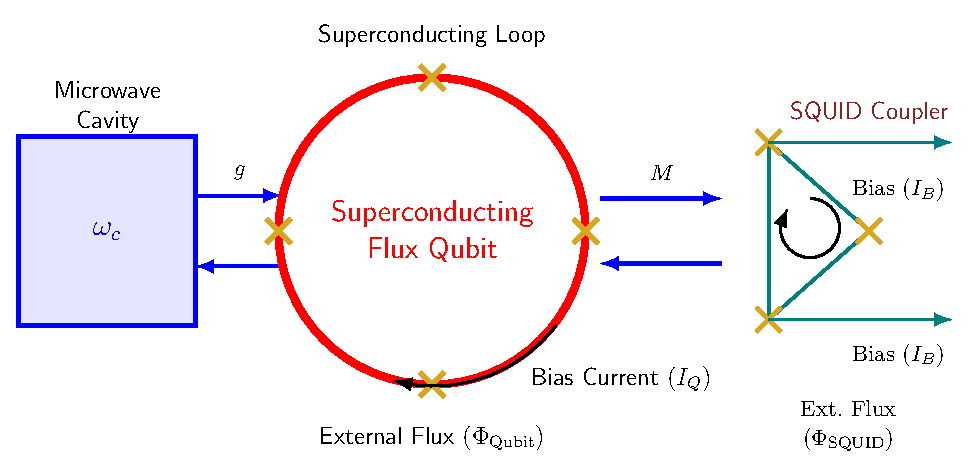
\includegraphics[width=0.7\columnwidth]{platform_flux_qubit.pdf}
\caption{Flux qubit platform. A superconducting loop with Josephson junctions forms a flux qubit (red) coupled to a microwave cavity (blue); external flux $\Phi_{\text{ext}}$ tunes the qubit frequency.}
\label{fig:platform_flux_qubit}
\end{figure}

\begin{figure}[hbt!]
\centering
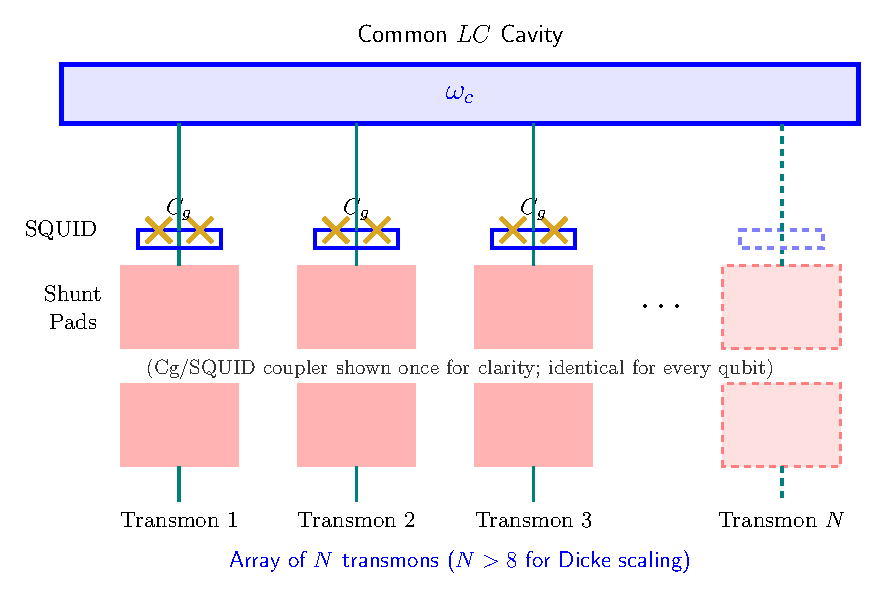
\includegraphics[width=0.7\columnwidth]{platform_transmon.pdf}
\caption{Transmon platform. An array of transmon qubits (red) capacitively coupled to a common $LC$ cavity (blue) via tunable couplers $C_g$.}
\label{fig:platform_transmon}
\end{figure}

\begin{figure}[hbt!]
\centering
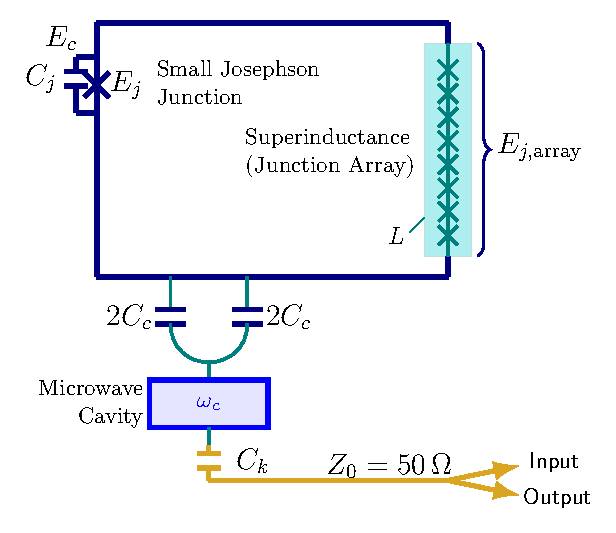
\includegraphics[width=0.7\columnwidth]{platform_fluxonium.pdf}
\caption{Fluxonium platform. High anharmonicity and long coherence enable operation at $\eta\sim\num{1.3}$ with $T_2>\qty{10}{\micro\second}$.}
\label{fig:platform_fluxonium}
\end{figure}

\textit{Staged program.} The experimental roadmap has three stages. Stage~1 ($N=\num{1}$, single qubit, flux-based CPW or 3D cavity) benchmarks the cavity-loss-augmented QFI against the first sampled single-qubit reference row (\qty{80.6}{\percent} at $\kappa/2\pi=\qty{0.6}{\mega\hertz}$); a 3D cavity at $\omega_c/2\pi=\qty{6}{\giga\hertz}$ is a candidate platform. Stage~2 ($N=\numrange{4}{8}$) tests the collective scaling exponent in the loss-controlled regime at the quoted $\eta=\num{1.15}$, without engaging the DCE modulation. Stage~3 ($N=\numrange{16}{32}$) simultaneously demonstrates collective dressing, DCE modulation, and the loss barrier; a 3D-cavity-based array is a candidate platform for the required low linewidth, but whether it can also provide the required collective coupling uniformity remains open. None of the three stages has been demonstrated end-to-end.

\subsection{Parameter-dependence scan}

\begin{figure}[hbt!]
\centering
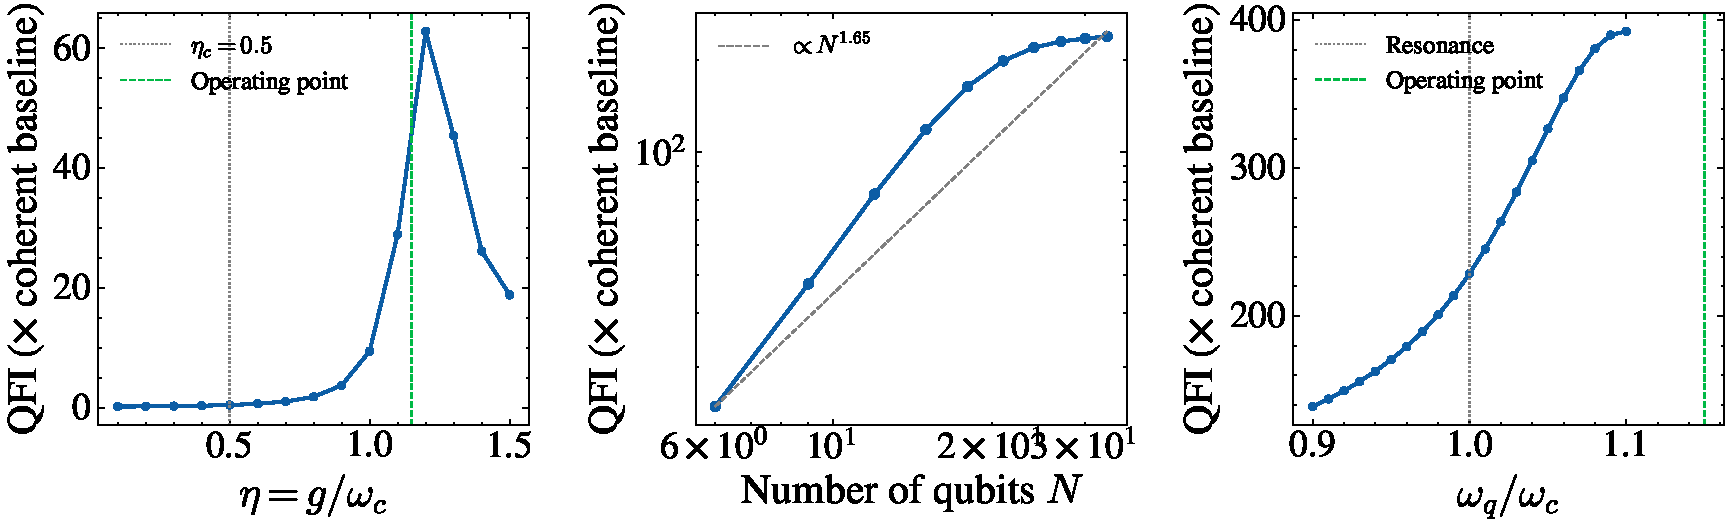
\includegraphics[width=.7\columnwidth]{figB_sensitivity.pdf}
\caption{Parameter sensitivity. (a) QFI vs $\eta$ at $N=\num{10}$, $n_{\max}=\num{15}$ (exploratory): the finite-size superradiant regime above $\eta_c=\num{0.5}$ shows a sharp onset, with $\sim\qty{7}{\percent}$ variation for $\eta>\num{1.1}$. (b) QFI vs $N$ at $\eta=\num{1.15}$, $\omega_q/\omega_c=\num{1.005}$: the super-linear $\propto N^{\num{2.22}}$ fit on $N\le\num{18}$ gives $N=\num{16}$ a factor $\sim\num{134}\times$. (c) QFI vs detuning at $N=\num{32}$, $n_{\max}=\num{35}$: maximum at $\omega_q/\omega_c=\num{1.10}$. Only panel (a) is exploratory; the retention claim refers to the detuning panel only.}
\label{fig:si_sensitivity}
\end{figure}

% ==================================================================
\section{Scope and limitations}
\label{sec:si_scope_B}

The results in this Supplemental Material are confined to the stated finite-dimensional models, drive conventions, and dissipation channels. They do not establish:

\begin{itemize}
\item loss immunity of the virtual-dressing state (the static result concerns parameter sensitivity of an undriven dressed state, not an extracted output);
\item a resource-normalized quantum advantage (photon-budget matching alone is insufficient);
\item an experimentally demonstrated QFI enhancement (the cavity HEOM cross-check shows a \qty{4.8}{\percent}--\qty{24}{\percent} model-comparison range at the physical linewidth);
\item two-level-emitter validity at the drive amplitudes of the main-text DCE QFI (all driven $d_e\ge\num{3}$ rows fail the \qty{1}{\percent} leakage criterion at the reference drive; safe operating windows exist only at reduced drive with correspondingly reduced enhancement);
\item a truncation-converged Dicke+DCE retention (the reduced-truncation range is \qty{2.6}{\percent}--\qty{16}{\percent} across $N_{\rm cav}=\num{6}$--$\num{24}$);
\item a thermodynamic or universal interrogation optimum (the crossover is model-specific);
\item a universal temperature threshold (the sampled crossover is tied to the explicit cavity frequency and bath model);
\item a general passive Floquet stabilizer (the finite-window screen retains boundary growth in low-loss resonant rows);
\item gauge-independent device predictions from the effective time-dependent Hamiltonian (the control convention must be specified across gauges).
\end{itemize}

\section*{Data availability}

Manuscript sources, deterministic analysis scripts, and the environment specification are publicly archived at \url{https://github.com/NanaEngo/Floquet-virtual-state-metrology-dce}.

\bibliographystyle{apsrev4-2}
\bibliography{references}

\end{document}
